%%%%%%%%%%%%%%%%%%%%%%%%%%%%%%%%%%%%%%%%%%%%%%%%%%%%%%%%%%%%%%%%%%%%%
% File Name:        rapport court 
%
% Description:      Rapport court du projet S5
%
% Note:             /
%
% Limitations:      /
%
% Errors:           None known
%
% Dependencies:     babel
%				    imta_core
%                   imta_extra
%                   isodate
%
% Author:          G. AOUICHAOUI - ghada.aouichaoui@telecom-bretagne.eu
% Encadrant:    JM. GILLIOT - jm.gilliot@imt-atlantique.fr
%
% University :     IMT Atlantique, Brest (France)
%
% TeX Environment: pdfLaTeX
%%%%%%%%%%%%%%%%%%%%%%%%%%%%%%%%%%%%%%%%%%%%%%%%%%%%%%%%%%%%%%%%%%%%

\documentclass{report}

\usepackage[francais]{babel}
\usepackage[francais]{isodate}

\usepackage{imta_core}
\usepackage{imta_extra}

\cleanlookdateon

\author{AOUICHAOUI Ghada}
\imtaSuperviser{Encadrant: GILLIOT Jean Marie}

\imtaAuthorShort{G. Ghada}
\date{\noexpand\today}
\title{Capturer ses expériences}
\subtitle{Rapport bibliographique - Projet 403}



\imtaSetIMTStyle

%%%%%%%%%%%%%%%%%%%%%%%%%%%%%%% 
%%%%%%%%%% DEBUT %%%%%%%%%% 
\begin{document}

	
\imtaMaketitlepage

\tableofcontents

\newpage

\chapter{Résumé}
Ce rapport est destiné à présenter le projet P-403: capturer ses expériences. Ce projet consiste à développer une application Android open source permettant à son utilisateur d'illustrer ses expériences et de stocker ses données numériques pour optimiser son apprentissage. Le contexte du projet et ses enjeux seront présentés dans ce rapport. Par la suite, une analyse du domaine et une étude bibliographique seront développés. Cette étude sera composée principalement de deux parties:

\begin{itemize}
    \item Les outils de collecte de données pour l'apprentissage qui existent déjà sur le marché et leurs spécificités.
    \item Les technologies envisagées pour développer notre application et les solutions retenues.
\end{itemize}.

À la fin du document vous trouverez une conclusion des choix faits pour le développement de l'application suivie d'une première version du plan de travail sous forme de GANTT \footnote{"Le diagramme de Gantt est un outil utilisé en ordonnancement et en gestion de projet et permettant de visualiser dans le temps les diverses tâches composant un projet." Wikipédia} qui contiendra tous les jalons du projet.
\chapter{Présentation générale du projet}



%% Contexte 
\section{Présentation du contexte}
Aujourd'hui l'enseignement en ligne connaît une croissance continue. Prenons l'exemple de l'IMT Atlantique qui met à la disposition de ses élèves plusieurs plate-formes en ligne (Moodle, Portail...). Ces plate-formes sont utilisées à de multiples fins:
\begin{itemize}
    \item Consulter des fichiers (cours, TPs, TDs, corrigés...)
    \item Remettre des devoirs
    \item S'inscrire aux examens
    \item Échanger avec les enseignants
    \item Passer des évaluations (QCM...)
    \item Consulter les résultats
    \item Déclarer des stages
\end{itemize}
Ceci conduit à l'explosion de la taille des données collectées. Pour exploiter efficacement ces données il a fallu avoir recours au Big Data en l'adaptant au domaine de l'éducation et de l'apprentissage: ceci s'appelle \emph{Learning Analytics}.\\ 
Cette discipline permet de gérer le volume, la variété et la rapidité de génération de ces données afin  de bien comprendre le comportement des apprenants et d'améliorer leur formation.\cite{ref1} 
\\
\\
Aujourd'hui \emph{Learning Analytics} est un domaine très prometteur, le problème de la protection des données à caractères personnels peut être soulevé.
En effet un des défis de cette technologie est de gérer l'accès et la sécurité des données rassemblées.
Pour pallier à ce problème, plusieurs entreprises se sont orientées vers la procuration d'une gestion personnelle des données par les utilisateurs eux mêmes; chaque apprenant est responsable de ses données et est libre de les partager avec les autres ou de les conserver pour lui même.
\\
Comment adapter ces solutions dans le domaine de l'éducation? 
Et comment proposer un service simple et fiable qui permet à l'apprenant de conserver ses expériences, de les exploiter efficacement et d'avoir un accès permanent à ses données?


%% Set up
\section{Reformulation du sujet}
Dans ce contexte, l'équipe SEDELA (Self Data for
Enhancing Learner Autonomy) piloté par Jean-Marie Gilliot et Serge Garlatti propose ce projet. L'objectif est de développer une application Android open source. Cette application aura pour finalité de permettre à l'apprenant, n'importe où et n'importe quand, de garder une trace de ses expériences d'apprentissage. Cette trace peut avoir plusieurs formes: texte, photo, vidéo... 
\\

Il pourra ensuite commenter ses expériences et rajouter des tags. Le tout sera sauvegardé, avec la géo-localisation et la date, dans un espace personnel réservé à l'utilisateur.

L'application lui offre aussi la possibilité de consulter toutes ses expériences et de les filtrer par rapport à plusieurs paramètres (la date, la localisation, des mot-clés...).
\\

En réalité, la formation de l'individu ne se limite pas au cadre scolaire ou jusqu'à l'obtention d'un diplôme. Tout au long de sa vie l'individu ne cesse d'apprendre et de se former. Pour cette raison, notre application s'adresse à tout apprenant indépendemment de son âge et de sa formation. 
\\

Chaque apprenant sera capable de rassembler ses données d'apprentissage pour les analyser, les partager avec une communauté de son choix ou tout simplement pour garder une preuve d'apprentissage.
\\ 

En effet, l'utilisateur se connectera à notre application où il aura accès à une première page qui lui permettra de prendre une photo, vidéo ou écrire du texte. Il donnera ensuite un titre à son expérience. L'application ajoutera la date et la géo-localisation. Il pourra ensuite enregistrer cette expérience qui s'ajoutera à la liste d'expériences qu'il a déjà capturé.
\\

L'application garantira un accès rapide et simple à cette liste et facilitera l'ajout de nouvelles expériences.
\\
En utilisant des logiciels open source, l'application sera libre à la distribution, son code source sera ouvert au public pour être modifié et exploité. En effet, le prototype sera ouvert (open source).


%% Sectioning
\section{Enjeux}
Le numérique se diffuse rapidement et profondément dans tous les secteurs qui doivent se transformer sous la pression de la mobilité, de l'Internet des Objets (IoT), de l'intelligence artificielle (IA) et du Big Data.
\\

Mais ceci n'empêche pas une grande \og crise de confiance \fg   dans le secteur du numérique: 60\% des internautes n'ont pas confiance dans l'usage d'Internet. \cite{ref2}
\\

Le secteur de l'éducation, n'est pas à l'abri de cette problématique. Plusieurs domaines d'activités du milieu universitaire sont concernés par la protection des données à caractère personnel. En effet l'utilisation de plusieurs plateformes, développées en interne ou fournis sous un contrat (Software as a service) qui traitent les données des étudiants à des fins de recherche scientifique ou autre, peut toucher au droit fondamental de la protection de la vie privée.
\\ 

Cet enjeu a conduit au développement de plusieurs applications et logiciels qui proposent le stockage de données en toutes sécurité et en respectant leur confidentialité. Par contre d'autres problèmes sont apparus:   
\begin{itemize}
    \item plate-formes payante
    \item accès réservés à une communauté bien réduite (Realto..)
\end{itemize}

Le but de ce projet est de permettre aux utilisateurs d'avoir le contrôle sur leur données et de pouvoir les exploiter librement.  Plus globalement cette application peut permettre aux établissements d'enseignement supérieurs d'utiliser les informations regroupées par leurs propres élèves et enseignants (après avoir demander leur accord) dans le cadre du partage de l'information et aussi de pouvoir les analyser dans le but d'optimiser et améliorer les formations qu'ils offrent.

%%%%%%%%%%%%%%%%%%%%%%%%
%%%   Analyse du domaine  %%%
%%%%%%%%%%%%%%%%%%%%%%%%
\chapter{Analyse du domaine}

%% Proto déjà existant

\section{Applications pour capter ses expériences}
\subsection{Daytripper v2}
\og Daytripper est né de la volonté d’accompagner les étudiants à la mobilité internationale (Erasmus). Je suis parti du constat suivant : nous apprenons beaucoup de choses et il est difficile à faire trace de son parcours, valoriser ce qu’on apprend et de le traduire en compétence et en talent. L’objectif était de leur apprendre à valoriser tout ce qu’ils vivent à l’étranger, leurs expériences à travers un « carnet de route » papier. \fg \cite{ref6}
\\

L'application Daytripper v2 permet à l'utilisateur de capter facilement ses expériences et de les garder dans un journal personnel et confidentiel.
\begin{center}
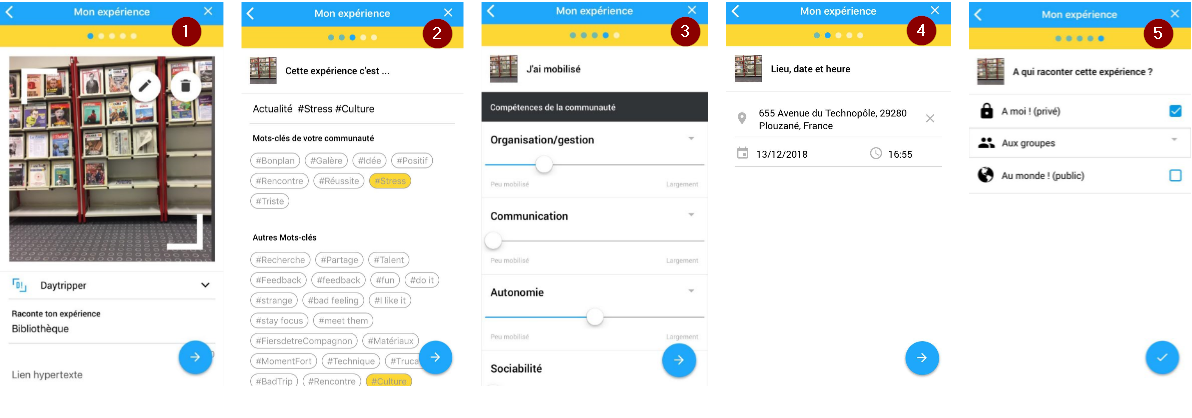
\includegraphics[height=150pt]{daytrip.png}
\end{center}
\begin{figure}[H]
    \centering
    \caption{Capture d'écran du déroulement de la création d'une expérience avec l'application Daytripper v2}
    \label{fig:Daytripper}
\end{figure}
L'utilisateur a aussi le choix de les partager au grand public ou dans des groupes de son choix. Chaque groupe offre un service différent des autres.
Quelques exemples de groupes en relation avec la vie professionnelle:
\begin{itemize}
    \item DIA\#LOG: identifier ses compétences et valoriser ses atouts auprès de ses interlocuteurs
    \item OPEN STORE: parler de ses expériences, communiquer des expériences concrètes...
\end{itemize}
À la fin, l'application propose à son utilisateur une liste de toutes les expériences qu'il a pu capturer avec les dates et les titres.

\begin{center}
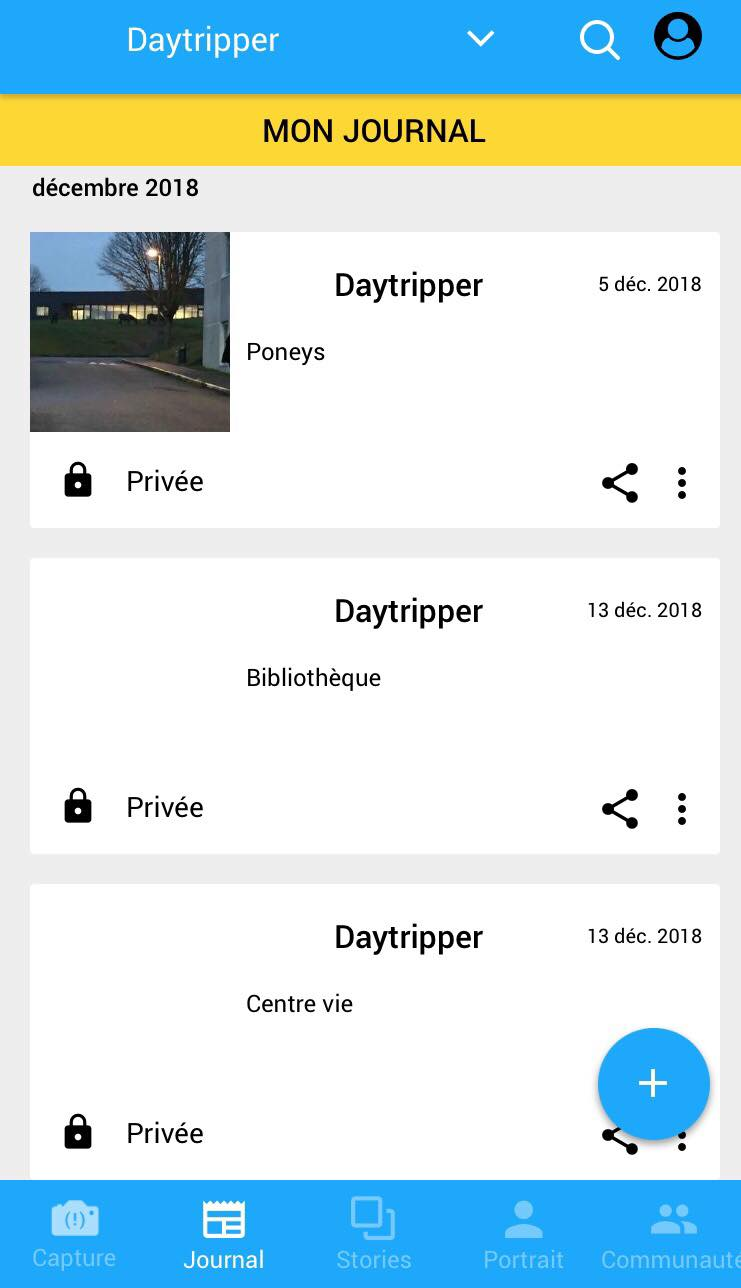
\includegraphics[height=150pt]{exp.jpg}
\end{center}
\begin{figure}[H]
    \centering
    \caption{Vue du journal dans l'application Daytripper v2}
    \label{fig:Daytripper}
\end{figure}

\emph{Daytripper} est une application ergonomique et simple d'utilisation. C'est un produit évolutif (plusieurs versions), ce qui donne une meilleure vitesse de chargement et une application moins lourde.




\subsection{Realto - La plateforme pour la formation professionnelle connectée}
La plateforme \emph{Realto}, qui doit son nom au pont vénitien \og Ponte di Rialto \fg, est aujourd'hui financé par le Secrétariat d'Etat à la formation, à la recherche et à l'innovation (SEFRI) et est développée par l'EPFL \footnote{École polytechnique fédérale de Lausanne} pour faire le lien entre l'expérience acquise sur le lieu de travail et ce qui est enseigné à l'école. 
\\

En effet, un apprenti est exposé à différentes expériences durant son apprentissage que celles ci soient faites sur le lieu de travail, à l'école ou aux cours inter-entreprises (réunissant des salariés de plusieurs sociétés et des particuliers).\\
Dans la réalité, ces expériences restent hélas sans connexion les unes avec les autres. Comment relier entre elles ces expériences et rapprocher réalité et théorie?

Realto offre à l'apprenti la possibilité de capturer ses expériences en un clic et de les conserver sous formes de photos, de vidéos, de commentaires ou de notes. Il pourra alors connecter ses expériences entre elles et en dégager une vue d'ensemble.\\

Il va aussi pouvoir les partager avec son formateur, ses collègues, ses enseignants d'école ou ses camarades de classe. Il pourra alors profiter des différents commentaires que ceux ci lui feront.\\
De son côté, l'enseignant pourra mener des activités d'apprentissage qui font appel aux expériences faites par les apprentis sur le lieu du travail. L'apprenti pourra aussi exploiter ses expériences pour constituer son dossier de formation qui deviendra un véritable ouvrage de référence sur ses apprentissages. Son formateur pourra examiner ce dossier quand il voudra, livrer son appréciation et se préparer à une discussion avec son apprenti.\\

\begin{center}
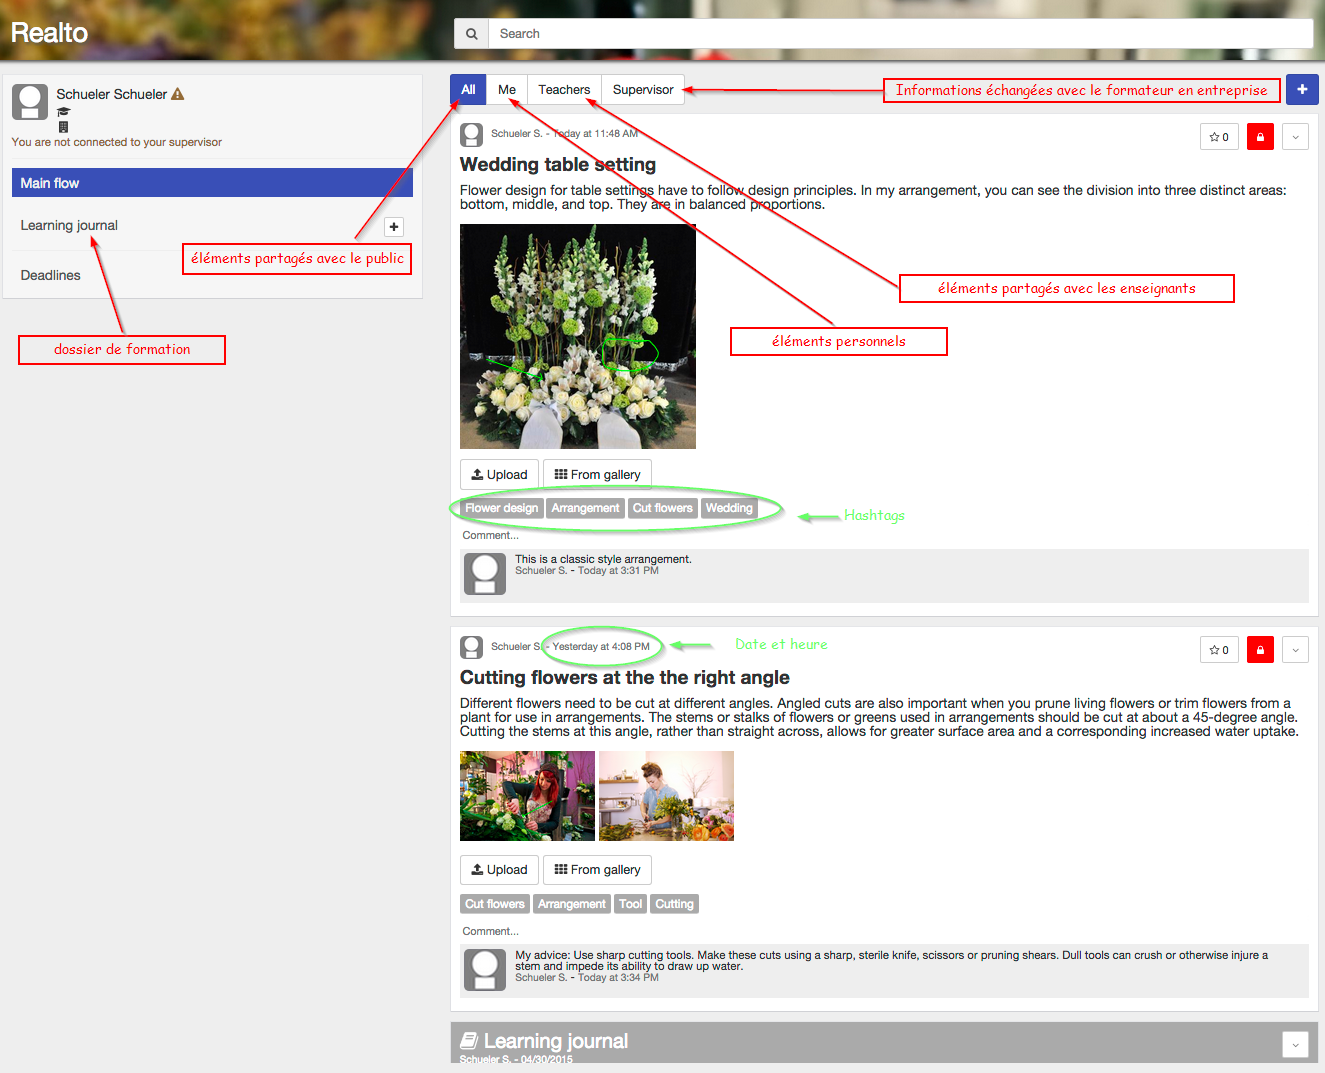
\includegraphics[height=300pt]{REALTO.png}
\end{center}
\begin{figure}[H]
    \centering
    \caption{Quelques éléments de l'interface de la plateforme REALTO}
    \label{fig:REALTO}
\end{figure}

À la différence des réseaux sociaux, \emph{Realto} permet à ses utilisateurs de contrôler en tout temps quelles informations ils veulent montrer et à qui.\\

\og A l’heure actuelle, Realto est déjà utilisé par 1440 apprentis, 230 enseignants et 240 formateurs de diverses professions.\fg \cite{ref8}

La plateforme offre aussi une version standard et d'autres versions plus adaptées aux besoins des professions partenaires.\\
\begin{center}
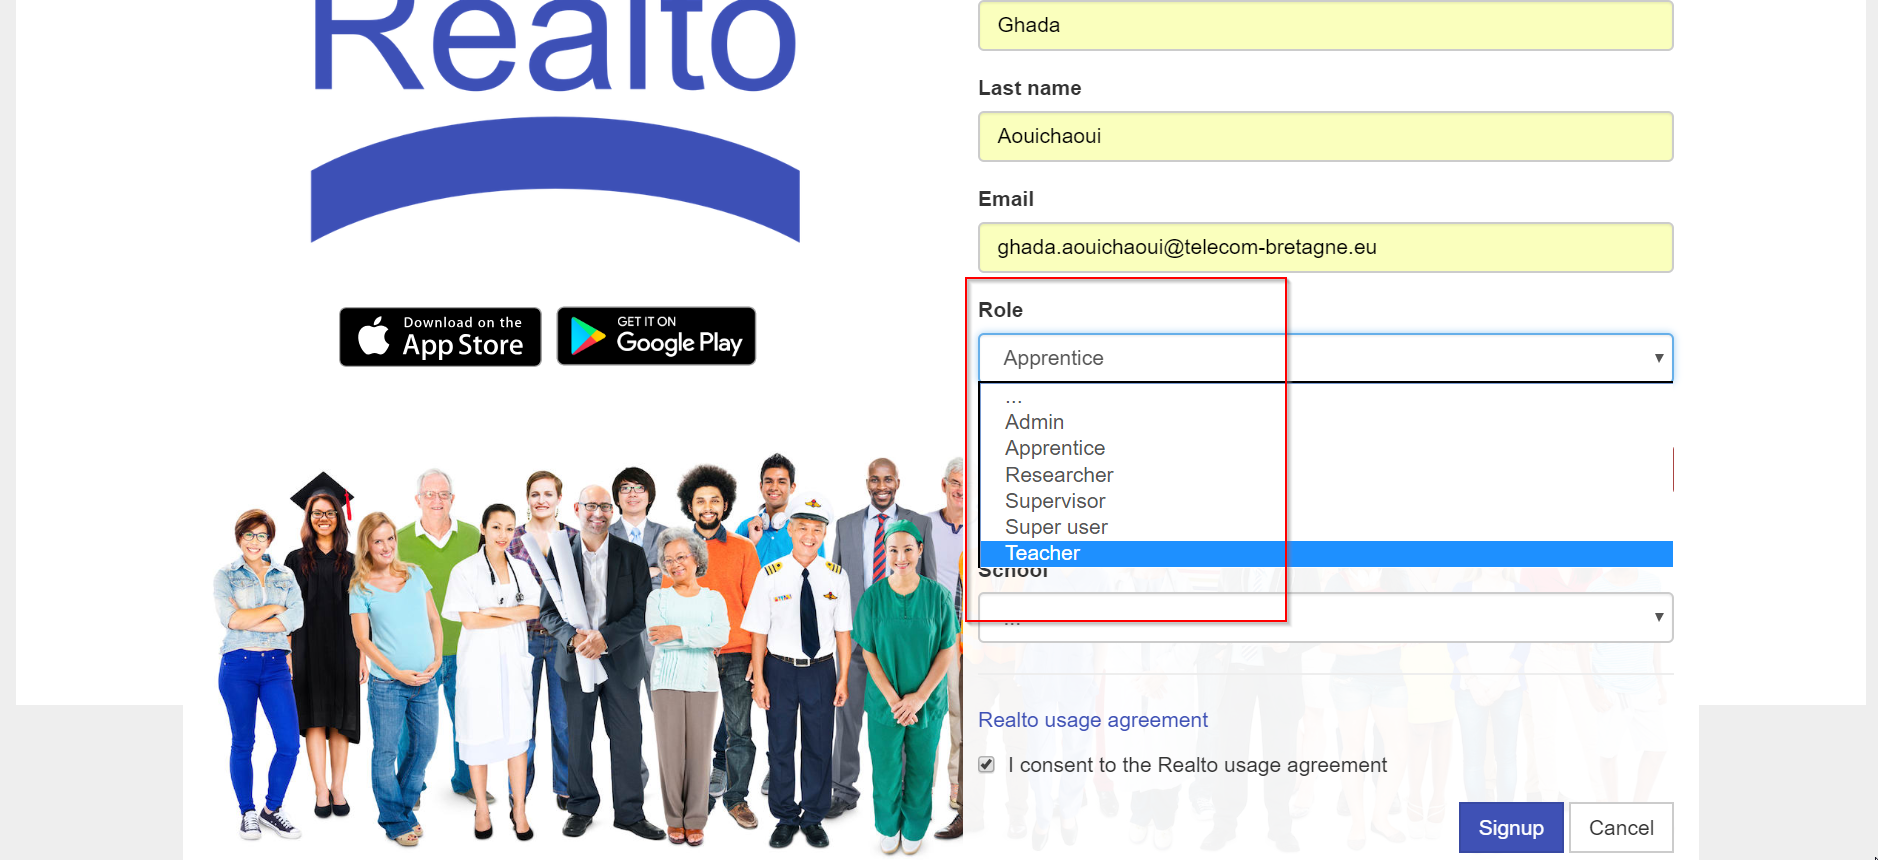
\includegraphics[height=200pt]{RoleLimite.png}
\end{center}

Realto est toujours peu adaptée au métier d'ingénieur. S'ajoute à cela le fait que ce logiciel est réservé à une communauté réduite (les étudiants, professeurs et personnels de l'EPFL...).

\subsection{Fonctionnalités offertes par notre application \emph{CaptureIT}}

Le projet CaptureIT permet de construire des passerelles entre la théorie d'une part et la pratique d'une autre part. Pour cela l'application offre les fonctionnalités suivantes :

\begin{itemize}
    \item Portfolio numérique: Mise en valeur des expériences capturées
    \item Géolocalisation: Utilisation des données de localisation du mobile pour situer les expériences sur un plan ou une carte
    \item Prise de photo simple et instantanée avec une possibilité de récupération des photos directement sur son smartphone
    \item Création d'un profil personnel pour l'utilisateur
    \item Rajout de notes personnelles et de  \og Hashtags\fg  pour décrire l'expérience
    \item Stockage des données récupérées par l'application sur le cloud personnel \texttt{Cozy} \footnote{Fonctionnalité gérée par l'équipe du projet 402 (décrite dans la section suivante)}
    \item Création d'une architecture de réseau où chaque utilisateur pourra partager ses expériences avec sa \og communauté \fg
    
\end{itemize}

\subsection{Lien avec le projet P402 - Collecter ses preuves d’apprentissage}
Dans le même contexte, \og ce projet se positionne dans une perspective de maîtrise des données d'apprentissage par les apprenants eux-mêmes, et donc avec
une dimension de gestion de données personnelles.\fg \footnote{Résumé du projet P402 sur http://projets.telecom-bretagne.eu }\\
Le rendu de ce projet est un prototype de portfolio qui contiendra des preuves d'expériences de l'apprenant. Ces données seront récupérées via des connecteurs et stockées dans une bases de données basée sur un système de cloud personnel (cozy). \footnote{"Cozy est une plateforme auto-hébergée, extensible et open source de cloud personnel." Wikipédia}\\
Ces données d'apprentissage seront collectées de différentes sources dont l'application CaptureIT. En effet toutes les expériences capturées par le biais de notre application seront exportées et stockées dans le portfolio décrit précédemment. 


\section{Outils de réalisation de l'application Android}
\subsection{Choix des langages de programmation}
Avant le début du développement de l'application mobile, un choix du langage de programmation utilisé doit être fait.\\
Plusieurs choix sont possibles, une brève analyse (les avantages et inconvénients) de quelques langages populaires est faite ci-dessous.
\subsubsection{Java}
Quand il s'agit de développement Android, la première et la plus populaire des solutions est Java. Java est le langage officiel du développement Android: il est soutenu par Google et la plupart des applications publiées sur le play store sont construites avec Java.\\

+Avec l'IDE \footnote{IDE: Integrated Development Environment} Android Studio, tous les outils de développement, débogage, affichage.. seront disponibles et facilement accessible dans un seul endroit.\\*

+Grâce au soutien de Google, il y aura accès à une variété de tutoriels, une documentation très fournie, un grand nombre de librairies...\\

-Langage plutôt compliqué à maîtriser: Android est de base un langage orienté objet avec des notions de constructeurs, exception.. Ajouter à cela un langage comme Java pourrait rendre le code illisible pour des développeurs débutants. Il requiert aussi des connaissances en Gradle, XML...\\
\textit{Java n'est pas le langage le plus adapté pour se lancer dans l'univers du développement Android. Continuons alors l'exploration d'autres langages.}
\subsubsection{C/C++}
+C/C++ est pris en charge par Android Studio avec le Android NDK. Ce qui signifie que l'application développée ne sera pas exécutée sur une machine virtuelle mais directement sur l'appareil. Cela offre un plus grand contrôle sur la mémoire, élément important lors du développement des applications intensives (jeux vidéo 3D par exemple).\\

-L'utilisation de C/C++ sur Android Studio peut être difficile à installer, introduit beaucoup de bugs et est peu flexible.\\

\textit{ Le choix du langage C/C++ pourrait être intéressant dans le cas de développent d'applications intensives. Mais ce n'est pas le cas de notre projet.}

\subsubsection{C\#}
C\# est une version plus simple, purement orienté objet de C/C++ développée par Microsoft. Comme Java, c'est aussi un langage \og garbage collected \fg \footnote{Permet le recyclage de la mémoire allouée puis inutilisée}\\

+Plus moderne que Java; syntaxe plus propre.\\

+Combiné avec un \og Game Engine \fg \footnote{fournit les calculs de physique et de géométrie }, c'est un outil simple et performant pour le développement des jeux vidéo. \\

-Moins performant pour le développement des fonctionalités de base d'Android.


\subsubsection{PhoneGap (HTML, CSS, JavaScript)}
C'est un framework basé sur Apache cordova.\\

+Il permet de développer des applications mobiles en s'appuyant sur les langages de développement de sites Web: HTML, CSS, JavaScript.\\

+PhoneGap Developper App permet l'aperçu immédiat des modifications apportées à l'application en cours de développement sur la plate-forme mobile.\\

+Il n'est pas limité au développement Android, mais aussi pour les plateformes iOS, Windows Phone.\\


\textbf{Conclusion: Même si PhoneGap ne présente pas du vrai développement Android (la seule partie développement sera la partie JavaScript), ce langage est bien adapté à notre projet. En effet, pour développer les fonctionnalités décrites ci dessus, ce langage semble être le plus intéressant.}


\subsection{Outil de développement: Software et Hardware}
Maintenant que le choix des langages de programmation est fait, il va falloir installer les différents outils logiciels et matériels pour pouvoir se lancer dans l'étape du développement.\\
P.S: Les étapes qui suivent correspondent à une installation sous Windows et pour la plateforme Android.
\subsubsection{Outils logiciels}
\begin{itemize}
    \item Installation de la CLI \footnote{Command-Line Interface} de Apache Cordova: pour cela il faut télécharger et installer Node.js (permettant l'exécution de JavaScript coté serveur) et ensuite lancer la commande:
    \begin{center}
        \texttt{npm install -g cordova}\\
    \end{center}
    
    \begin{center}
    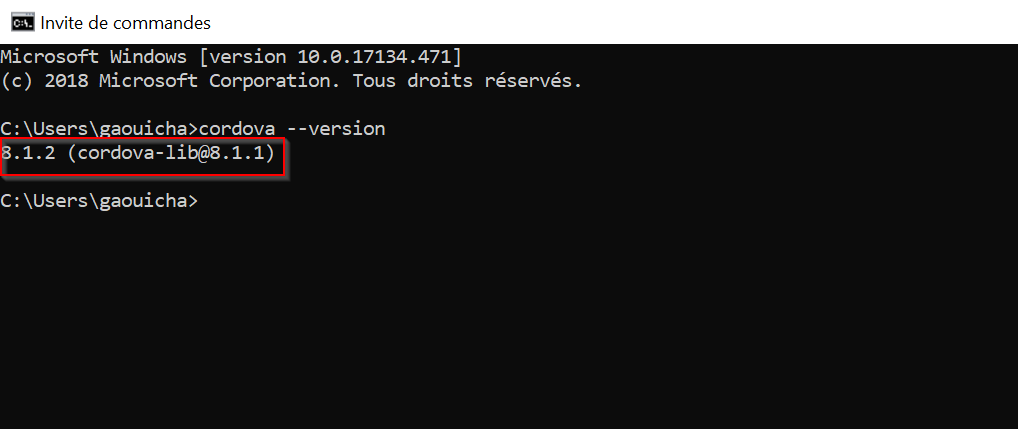
\includegraphics[height=200pt]{cordova.png}
    \end{center}
    \begin{figure}[H]
        \centering
        \caption{version de Cordova utilisée pour le développement de l'application}
        \label{fig:cordova}
    \end{figure}

    \item Installation du SDK \footnote{Software Development Kit} qui va permettre la compilation, le débogage et les tests sur Android: ceci correspond à l'installation de 3 pré-requis:
    \begin{itemize}
        \item Le JDK \footnote{Java Development Kit} qui correspond au bon système d'exploitation (dans ce cas Windows 64)
        \item Le SDK d'Android
        \item Apache ANT: vise à automatiser les opérations répétitives du développement de logiciel (compilation, la génération de documents..)
    \end{itemize}
    
    \begin{center}
    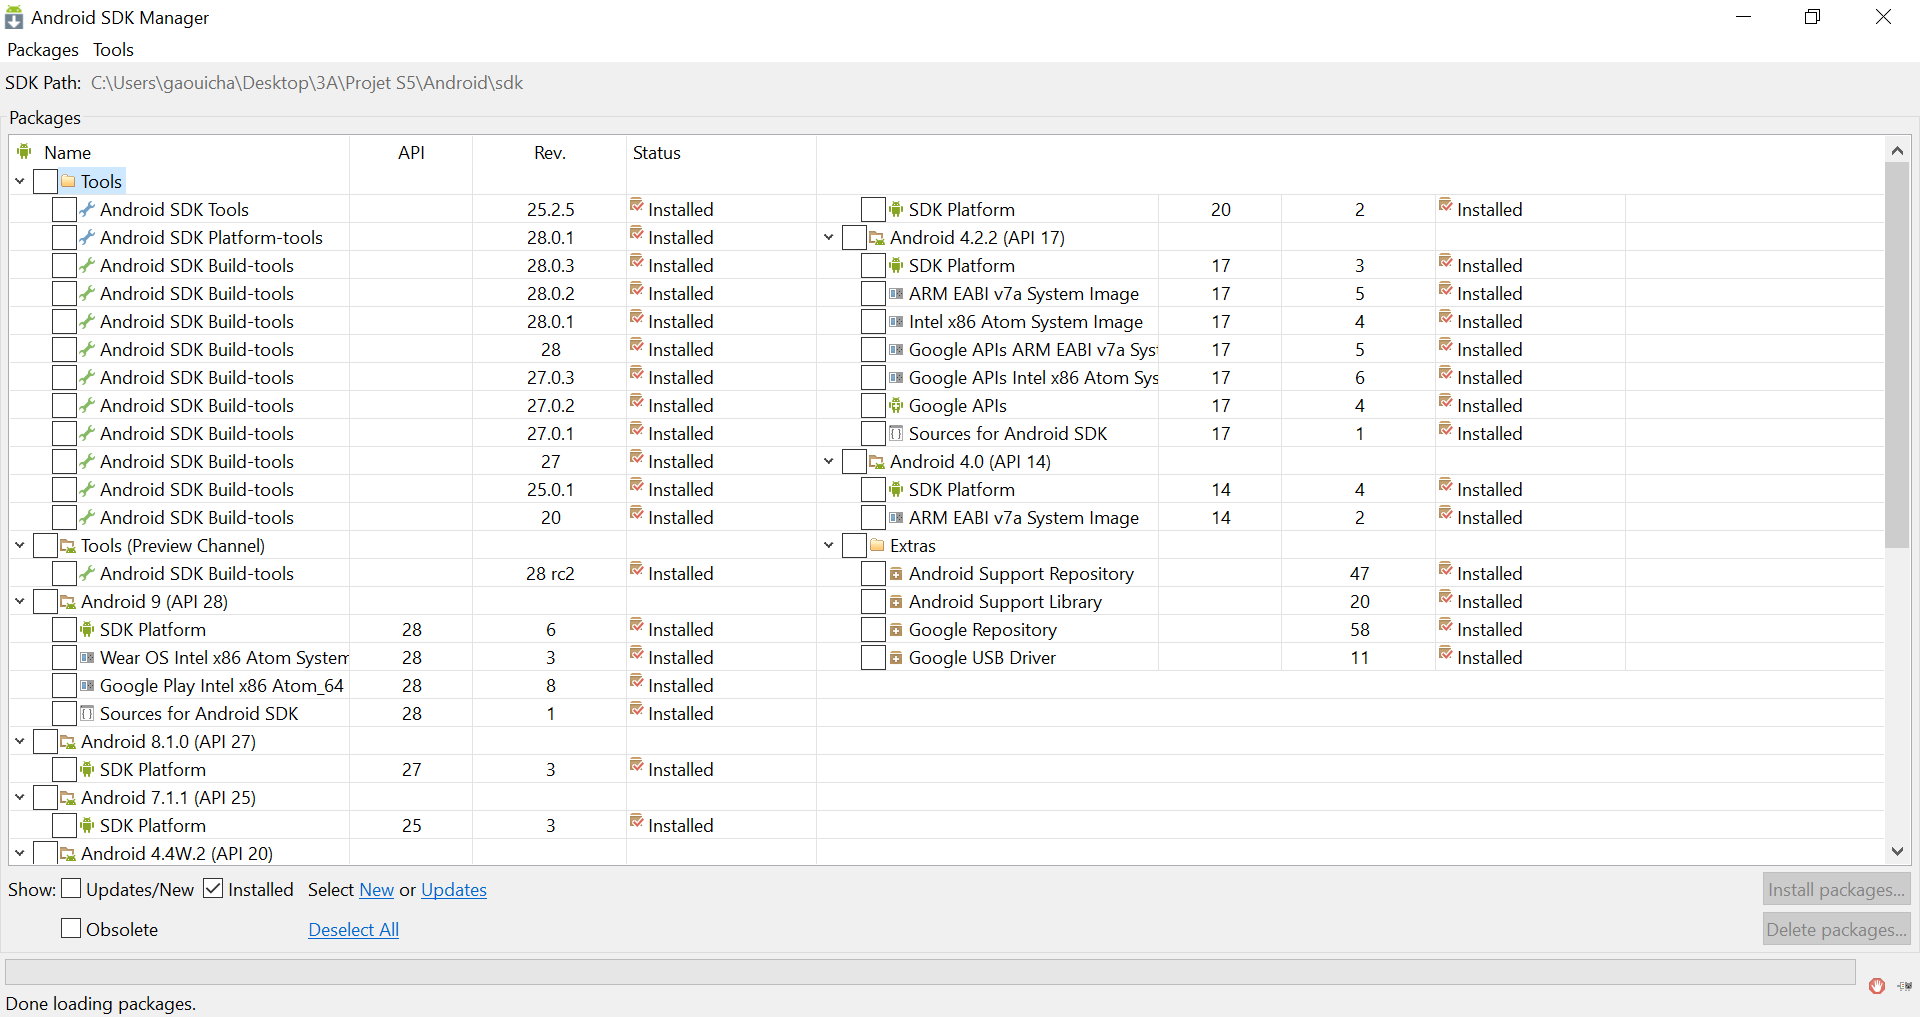
\includegraphics[height=250pt]{SDK.png}
    \end{center}
    \begin{figure}[H]
        \centering
        \caption{Android SDK AVD manager}
        \label{fig:SDK}
    \end{figure}
\end{itemize}


\subsubsection{Outils matériels}
La programmation sera effectuée sur un ordinateur dotée des capacités suivantes:
\begin{itemize}
    \item Marque: ASUS
    \item Microprocesseur: Intel core 
    \item RAM: 8,00 Go
    \item Système d'exploitation: 64 bit, processeur x64
    \item Disque dur: 237 Go
\end{itemize}
Les tests seront effectués directement sur une tablette tactile Android qui a les caractéristiques suivantes:
\begin{itemize}
    \item Écran: 10 pouces
    \item Processeur: Qualcomm MSM8228
    \item Espace total: 9,82 Go
\end{itemize}


%% Styling
\section{Réalisation d'un prototype ouvert: défis et solutions}
L'open source est l'avenir de l'innovation. En effet les logiciels développés en open source sont continuellement mis à jour par leurs utilisateurs. C’est ce qui fait que le rythme d’innovation open source est nettement plus soutenu que pour les logiciels propriétaires.\\


Dans ce contexte, l'application à développer sera ouverte et sous licence libre. 

Dans le cadre du projet, un problème se pose au niveau des appels des API cartographiques (pour assurer la fonctionnalité de géolocalisation dans CaptureIT). En effet le service de cartographie le plus connu, Google maps n'est pas open source et son API est devenue payante \footnote{depuis juillet 2018}. Il faudra alors trouver des alternatives.\\


\texttt{OpenStreetMap} est l'alternative Open Source la plus connue à Google Maps. "OSM" propose des cartes complètes, exportables et mises à jour par une communauté active.\\

Afin de pouvoir utiliser les cartes d'OSM dans une application Android, plusieurs librairies sont disponibles:

\begin{itemize}
    \item osmdroid: une bibliothèque Android qui fournit des outils/ des vues permettant d'interagir avec OSM-Data \cite{ref9}
    \item Mapsforge: une bibliothèque de cartes vectorielles écrite en Java prenant en charge Android et JRE. Il fonctionne en rendant les données osm à la demande (sur le périphérique) et hors ligne.
\end{itemize}

Par souci de simplicité, la solution retenue est la bibliothèque \emph{osmdroid}. En effet, CaptureIT localise juste les expériences capturées sur une carte. Il n'est donc pas utile de pouvoir modifier ou manipuler les cartes. 







\chapter{Conclusion de l'analyse}
Après avoir étudié différents environnements de développement j'en tire la conclusion suivante:
je vais implémenter l’application en utilisant le framework Apache Cordova qui se base sur des langages de programmation Web : HTML, CSS et JavaScript. \\
Bien qu'Android studio soit un environnement très riche et performant, devoir apprendre tout un langage natif Java pourrait être contraignant.\\

Concernant les différentes fonctionnalités de l’application, je me limiterai aux outils open source pour pouvoir avoir un prototype ouvert comme produit final. En effet pour la géolocalisation des expériences captées, j’utiliserai la bibliothèque d’OpenStreet-Map : osmdroid qui fournit un suivi de l’emplacement, le dessin de formes.. en ligne et hors connexion. \\
En ce qui concerne le design des différentes pages de l’application, j'ai réalisé à l’aide de l’outil FIGMA \footnote{un outil collaboratif pour le design d'interface}, un premier croquis représenté ci-dessous:

\begin{center}
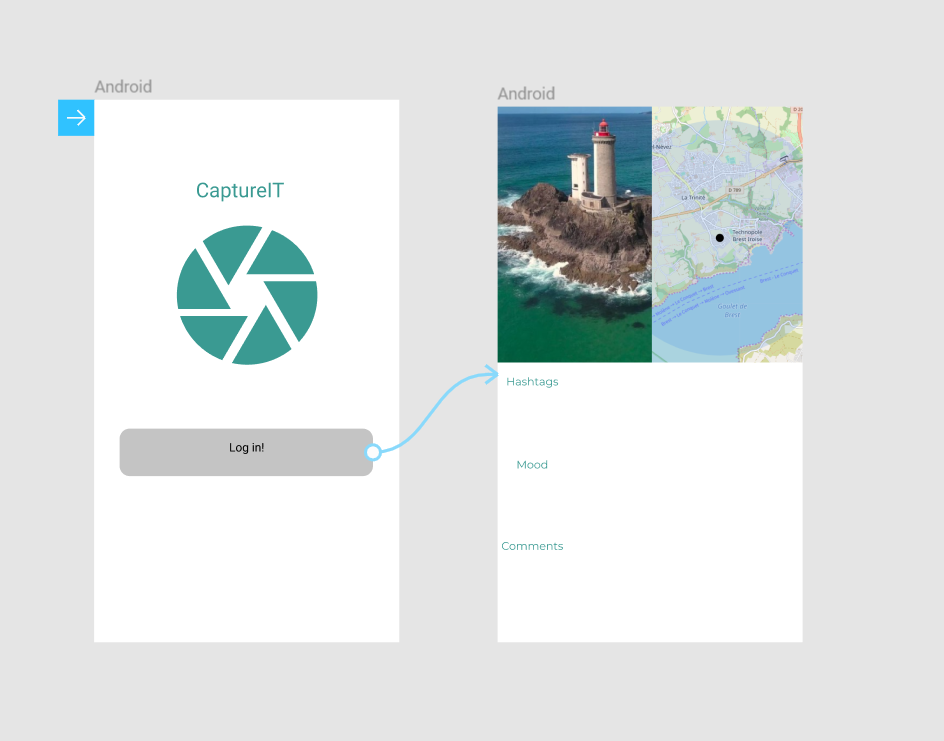
\includegraphics[height=150pt]{CaptureIT.png}
\end{center}
\begin{figure}[H]
    \centering
    \caption{Design de quelques vues de l'application à coder et le lien entre eux}
    \label{fig:CaptureIT}
\end{figure}

J'ai commencé ensuite à coder cette interface en HTML/CSS. \\

\begin{center}
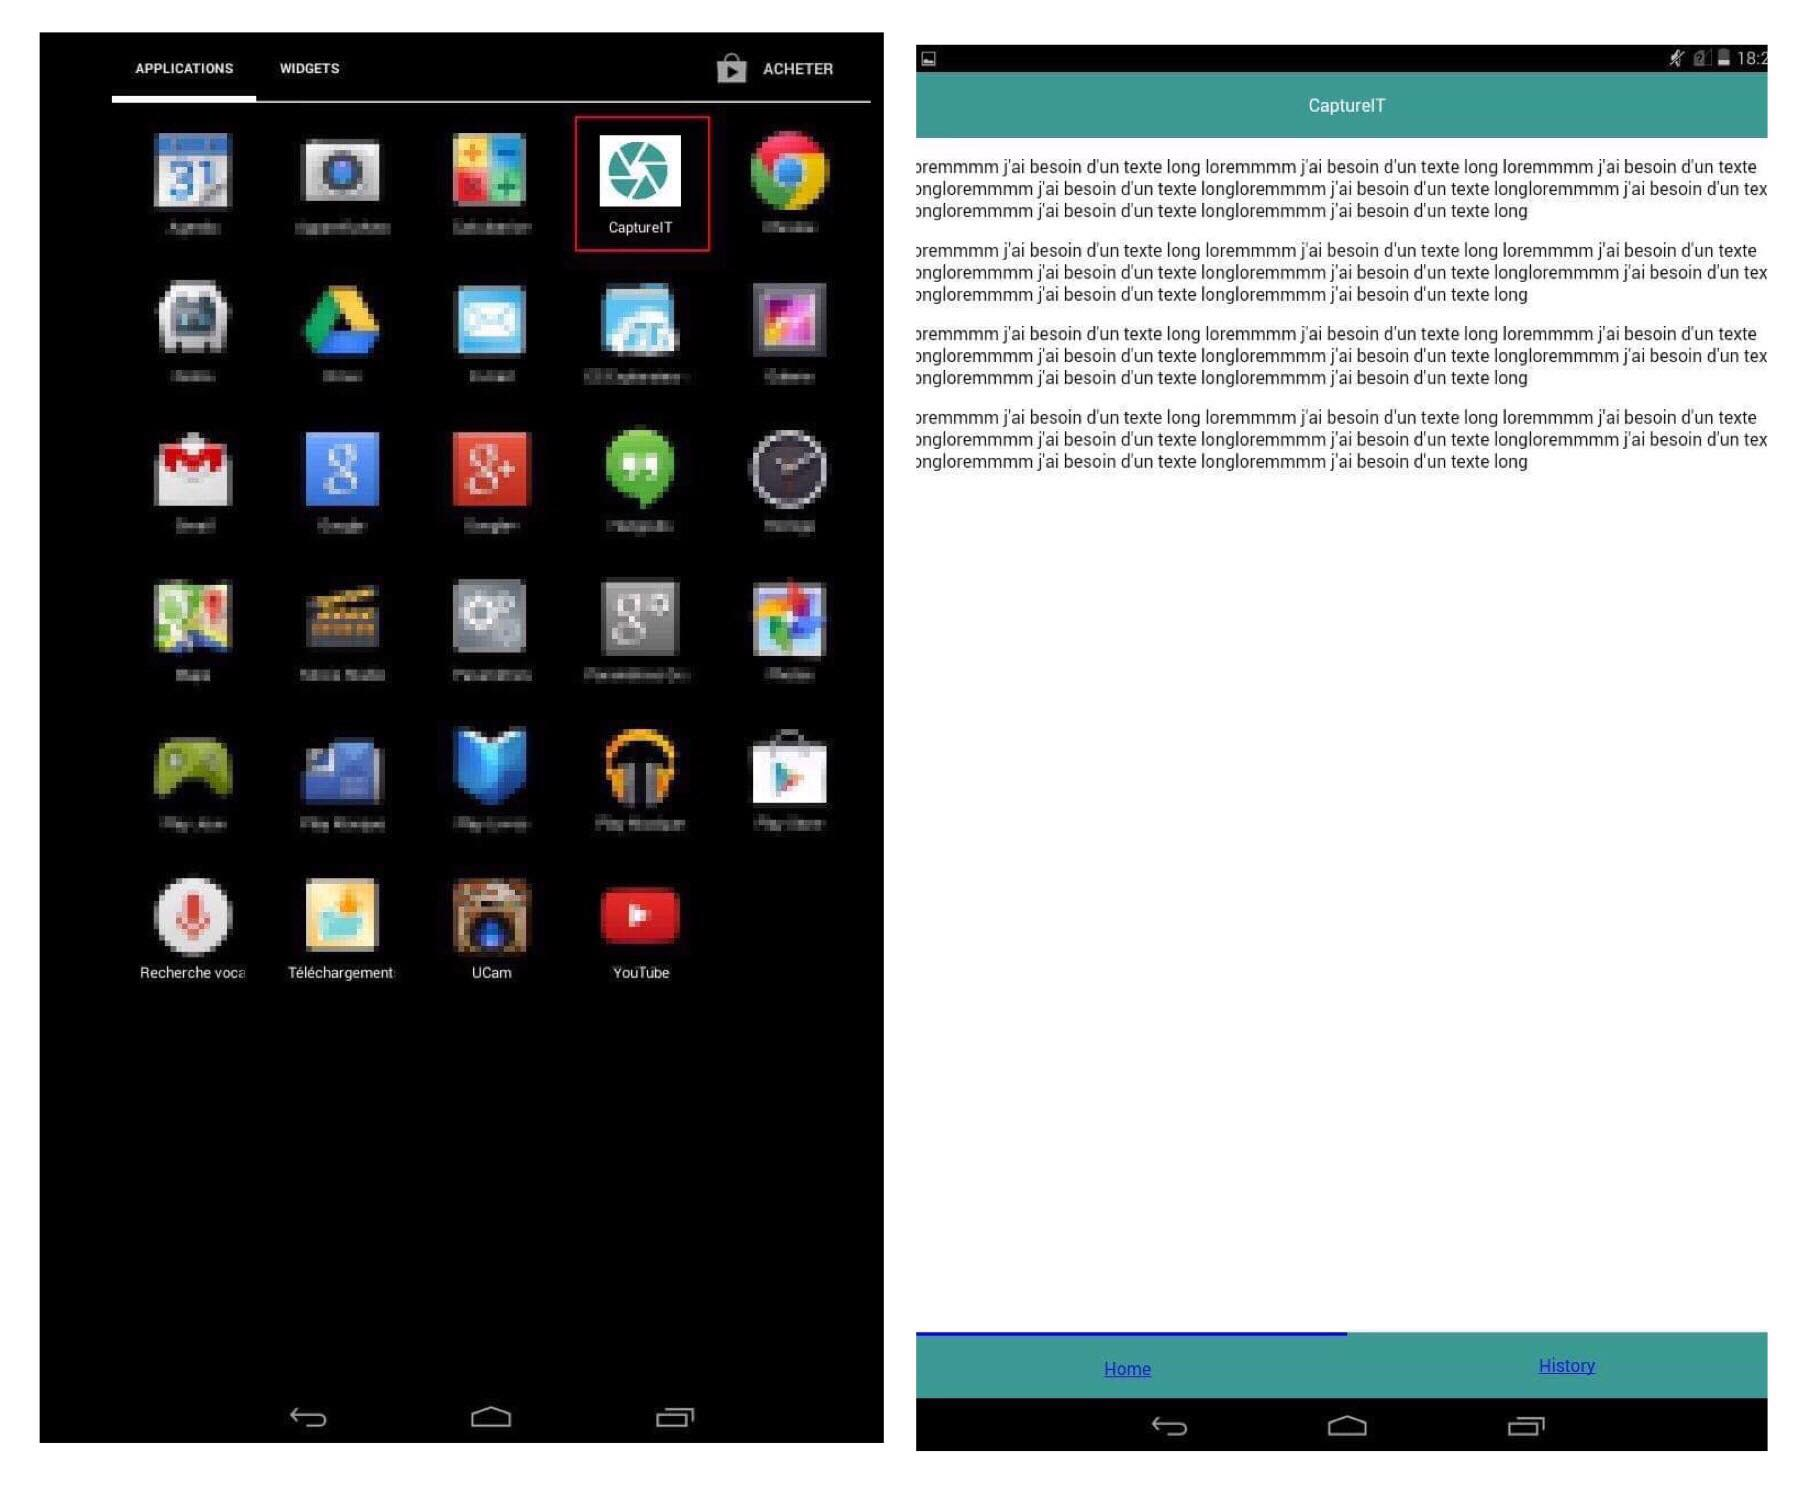
\includegraphics[height=200pt]{screen.jpg}
\end{center}
\begin{figure}[H]
    \centering
    \caption{Rendu du premier prototype de CaptureIT sur l'écran d'une tablette Android}
    \label{fig:CaptureIT}
\end{figure}





% List of environments
\chapter{Plan de travail}
Pour bien gérer l'avancement du projet, le développement de l'application sera fait en plusieurs étapes:
\begin{itemize}
    \item le squelette de l'application qui contiendra les tâches élémentaires (connexion...).
    \item les fonctionnalités qui permettront de prendre des photos, de les commenter, de les géolocaliser...
    \item un réseau dans lequel l'utilisateur pourrait partager, s'il le souhaite, ses expériences
\end{itemize}
J'aurai des prototypes à rendre tous les mois sous forme de code commenté sur le GitHub.\\
Mon objectif est d'avoir à la fin du projet une application capable de réaliser le scénario suivant:\\
Un apprenant se connecte à  l'application. Il arrivera sur une page où il pourra prendre une photo. Une fois la photo prise, il verra apparaître la date et la géolocalisation. Il pourra ensuite rajouter du texte et des tags en bas de la photo. Une fois il aurait rajouté tous les éléments nécessaires pour illustrer son expérience, il sera capable de l'enregistrer. Toutes les expériences capturées seront disponibles dans un espace personnel.
\\

Sur le diagramme GANTT ci-dessous, vous trouverez les différentes étapes.

\textbf{\begin{center}
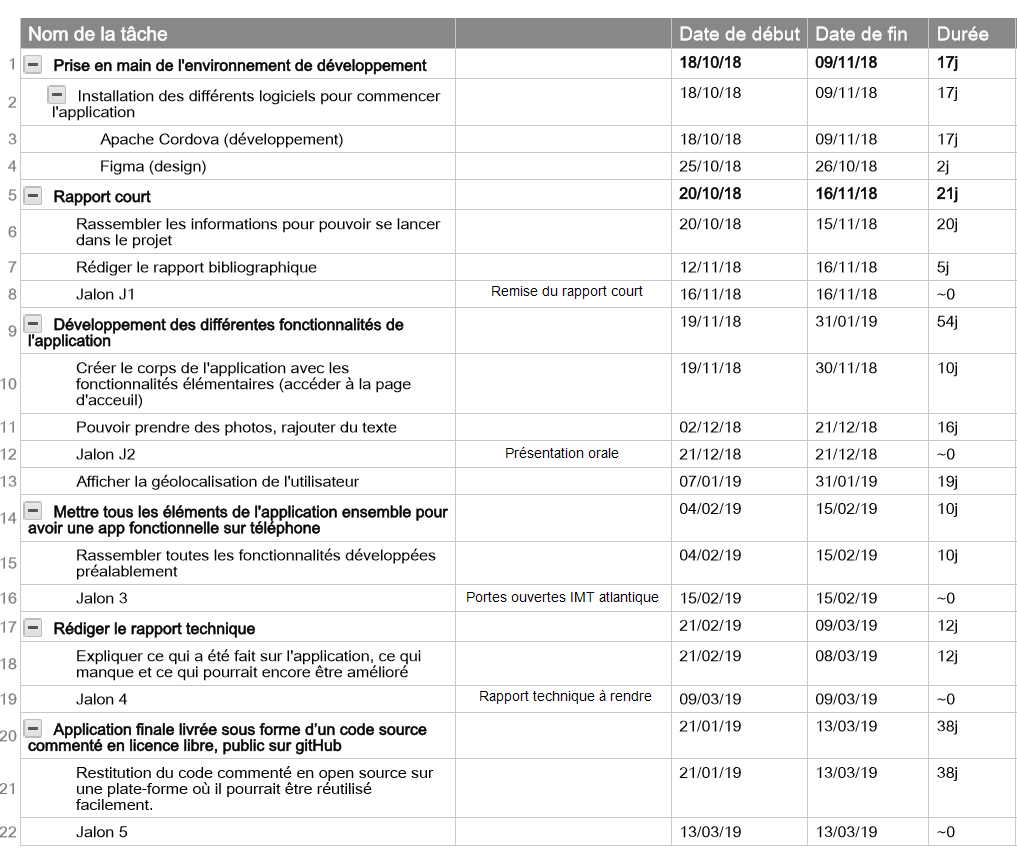
\includegraphics[width=400pt]{GANTT.png}
\end{center}
}
\begin{figure}[H]
    \centering
    \caption{GANTT chart}
    \label{fig:GANTT}
\end{figure}

\bibliographystyle{plain}
\bibliography{bibli}


\imtaMakeCover

\end{document}

%%%%%%%%%% END %%%%%%%%%% 
%%%%%%%%%%%%%%%%%%%%%%%%% 
